
\documentclass[../PianoProgetto.tex]{subfiles}

\begin{document}

\section{Pianificazione}
\label{sec:pianificazione}

	Di seguito saranno elencate le durate e le caratteristiche di ogni fase\g . I tempi sono stati pensati per permettere uno slack\g\ sufficiente, in modo da mitigare i rischi relativi alle tempistiche.
	
	\subsection{Fase A: Analisi}
	
	\textbf{Periodo: dal 2015-11-23 al 2016-01-22}

	Questa fase\g\ comincia con la presentazione in aula delle regole del progetto didattico e termina con la scadenza della consegna riguardante la \revisionedeirequisiti .

	Le attività sono le seguenti:
	\begin{enumerate}
		\item \textbf{scelta degli strumenti}: verranno scelti gli strumenti che saranno utilizzati per la stesura dei documenti e per il supporto;
		\item stesura \textbf{Norme di progetto}: dopo aver individuato gli strumenti si potrà procedere alla stesura del documento \textit{Norme di progetto v1.00}. Questo documento sarà utilizzato indipendentemente dal capitolato\g\ che verrà preso in appalto;
		\item \textbf{stesura documentazione}: in questa fase\g\ gli strumenti da utilizzare e le norme per scrivere un documento sono definite, quindi è possibile iniziare la stesura dei seguenti documenti:
		\begin{itemize}
		\item Studio di fattibilità: vengono valutati pro e contro di tutti i capitolati proposti e viene redatto il documento \textit{Studio di fattibilità v1.00}. Viene quindi scelto il capitolato\g\ da sviluppare;
		\item Analisi dei requisiti: viene steso il documento \textit{Analisi dei requisiti v1.00}. Prima e durante la stesura di questo documento verranno organizzati degli incontri con il proponente per consolidare i requisiti stesi o per chiarire le idee sui requisiti da stendere;
		\item Piano di progetto: si stende il documento \textit{Piano di progetto v1.00} per regolare le attività che il team\g\ dovrà svolgere;
		\item Piano di qualifica: si redige il documento \textit{Piano di qualifica v1.00} per fissare gli obiettivi di qualità e le strategie per perseguirli;
		\item Glossario: viene incrementato il file \textit{"Glossario.xml"} e steso in modo automatico il documento \textit{Glossario v1.00}.
		\end{itemize}
	\end{enumerate}
		\newpage
		\subsubsection{Diagramma di Gantt – Fase A}
			\begin{figure}[!h]
				\centering
				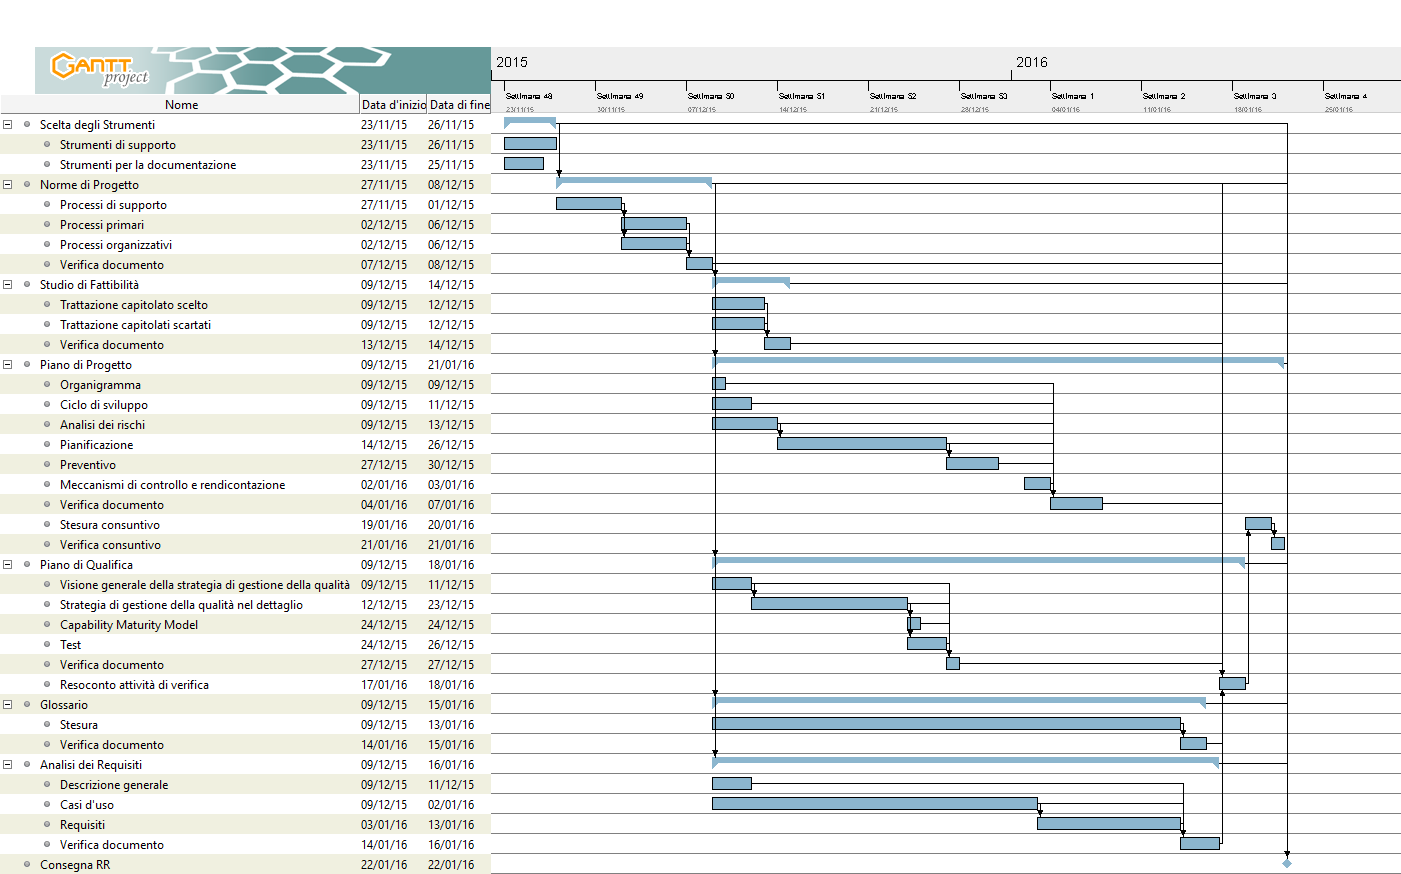
\includegraphics[width=\textwidth]{gantt_png/1-analisi}
				\caption{Gantt - Fase A}
				\label{fig:Gantt - Fase A}
			\end{figure}			
	
	\subsection{Fase AD: Analisi di Dettaglio}
		\textbf{Periodo: dal 2016-02-16 al 2016-02-22}

				Questa fase\g\ comincia al termine della fase\g\ A. È caratterizzata da un incremento di tutti i documenti redatti nella fase precedente e dalla correzione in base alle richieste e segnalazioni del committente e del proponente. Gli \analisti\ provvedono all'individuazione di nuovi requisiti e alla correzione dei requisiti segnalati, successivamente si provvede all'incremento di tutti gli altri documenti. Dopo aver aggiornato i requisiti, si terrà un incontro con il proponente per la loro verifica.
		\newpage			
		\subsubsection{Diagramma di Gantt – Fase AD}
			\begin{figure}[!h]
				\centering
				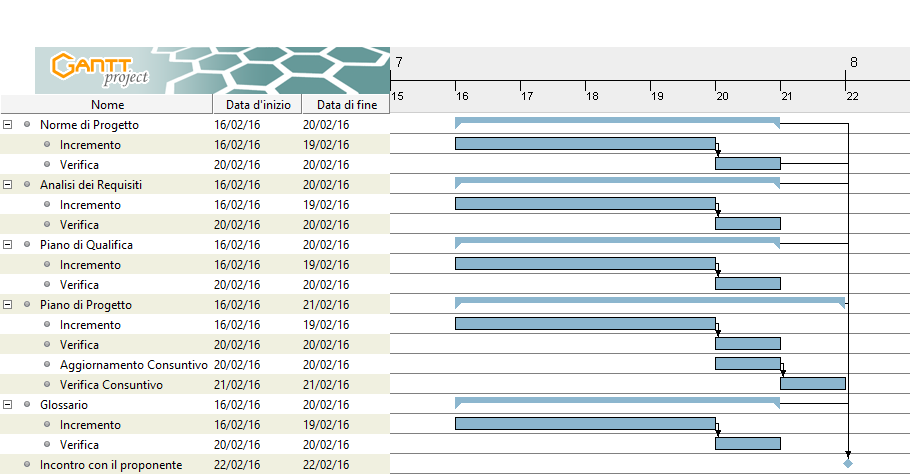
\includegraphics[width=\textwidth]{gantt_png/2-analisi_di_dettaglio}
				\caption{Gantt - Fase AD}
				\label{fig:Gantt - Fase AD}
			\end{figure}

	\subsection{Fase PA: Progettazione Architetturale}
		\textbf{Periodo: dal 2016-02-22 al 2016-03-14}
		
		Questa fase\g\ comincia con la fine della fase\g\ AD e termina con un incontro con il proponente per mostrare l'architettura logica prodotta. Le attività di questa fase sono:
		\begin{itemize}
			\item Norme di progetto: viene incrementato alle \normediprogetto\ per poi stendere il documento \specificatecnica . Successivamente dopo una verifica per fissare una baseline il documento diventerà \textit{Norme di Progetto v3.00};

			\item Specifica tecnica: questa attività caratterizza la Progettazione Architetturale. Il \progettista\ stende la \specificatecnica\ che contiene le scelte progettuali, ad alto livello, che il progetto dovrà avere. Saranno quindi descritti quali design pattern implementerà, l'architettura logica del software\g , i principali flussi di controllo, il tracciamento dei requisiti e i componenti hardware da utilizzare nei successivi test di sistema del prodotto;

			\item Glossario: viene fatto un incremento al \glossario\ aggiungendo tutti i vocaboli che si ritiene debbano essere inclusi. Viene successivamente fatta una verifica per fissare una baseline del documento che diventerà \textit{Glossario v3.00};

 			\item Piano di qualifica: l'incremento consiste nell'aggiungere al documento \pianodiqualifica\ i dettagli dell'esito della \revisionedeirequisiti\ e la parte della pianificazione dei test. Questa attività genererà, dopo una verifica e validazione, il file \textit{Piano di Qualifica v3.00};

			\item Piano di progetto: l'incremento che sarà fatto al documento \pianodiprogetto\ in questa fase\g\ consiste nell'apportare correzioni riguardanti la divisione delle attività e stilare il consuntivo di questo periodo. Dopo una verifica che fisserà una nuova baseline e la validazione il documento diventerà \textit{Piano di Progetto v3.00}.
						
		\end{itemize}
		
		\subsubsection{Diagramma di Gantt – Fase PA}
			\begin{figure}[!h]
				\centering
				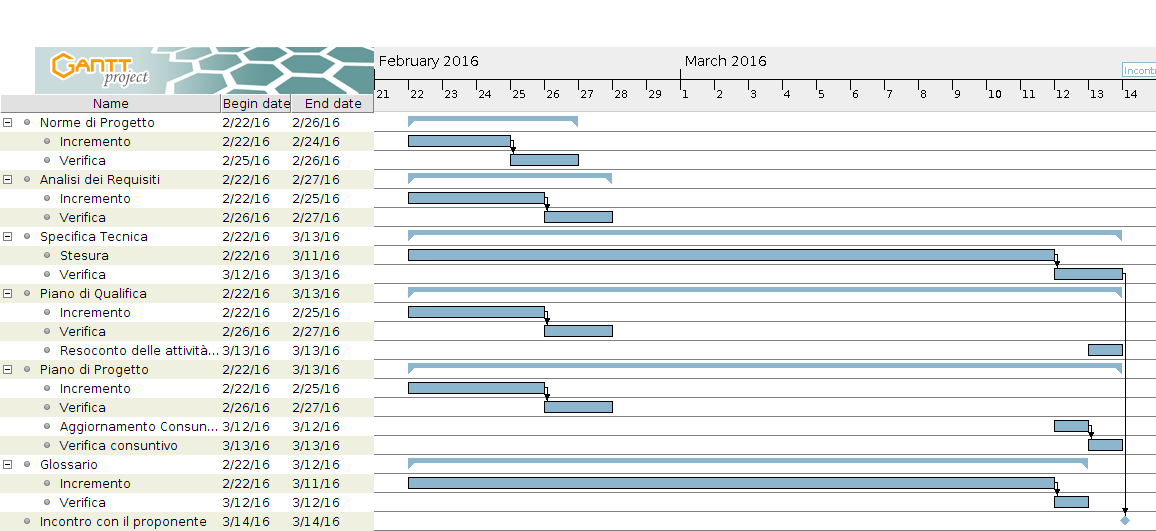
\includegraphics[width=\textwidth]{gantt_png/3-progettazione_architetturale}
				\caption{Gantt - Fase PA}
				\label{fig:Gantt - Fase PA}
			\end{figure}
			
	\subsection{Fase PDROB: Progettazione di Dettaglio e codifica dei Requisiti Obbligatori}
		\textbf{Periodo: dal 2016-03-15 al 2016-04-11}
		
		Questa fase\g\ inizia con la fine della fase\g\ PA e termina con la consegna della \revisionediprogettazione . Le attività di questa fase saranno le seguenti:
		\begin{itemize}
			\item Definizione di prodotto: viene steso il documento \textit{Definizione di prodotto v1.00}. Esso definisce la struttura interna del sistema e le relazioni tra i componenti del prodotto\g\ relativi ai requisiti obbligatori;

			\item codifica: con quest'attività inizia lo sviluppo da parte dei \programmatori\ dei requisiti obbligatori. Sarà dunque seguito quanto riportato nel documento \textit{Definizione di prodotto v1.00};

			\item incremento e verifica documenti: vengono eseguite modifiche ai documenti già scritti, dove necessario;

			\item Glossario: vengono aggiunti al \glossario\ i vocaboli dei quali si ritiene necessaria una definizione formale. Alla fine di questa fase\g\ viene quindi generato il documento \textit{Glossario v4.00}.
		\end{itemize}

		\subsubsection{Diagramma di Gantt – Fase PDROB}
			\begin{figure}[!h]
				\centering
				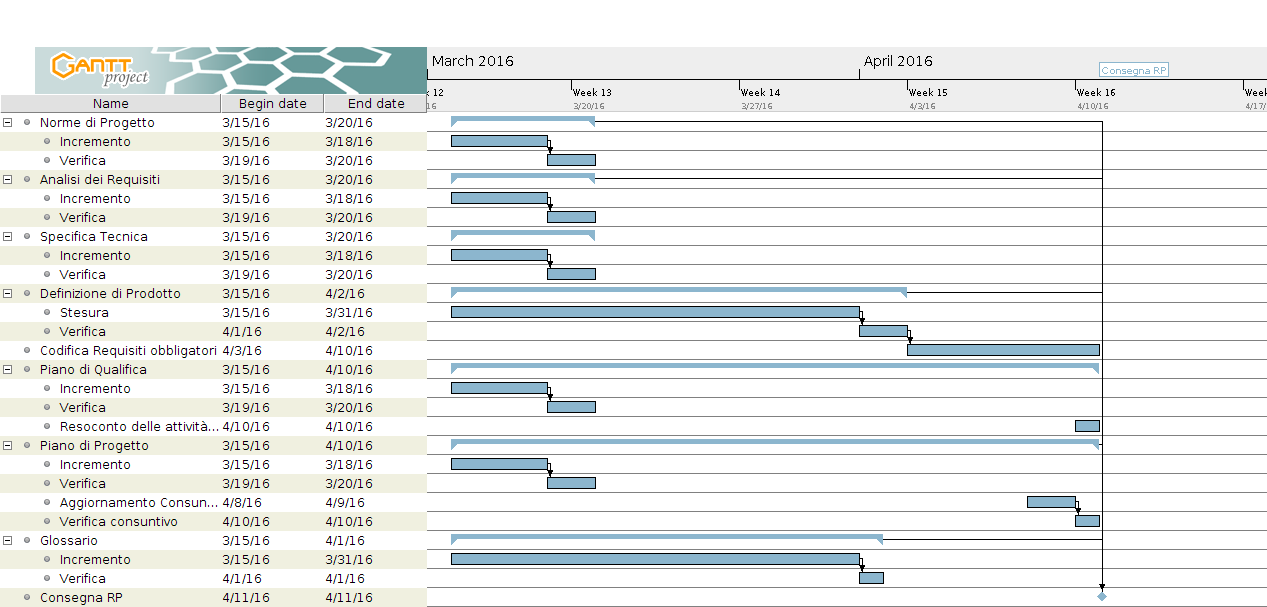
\includegraphics[width=\textwidth]{gantt_png/4-requisiti_obbligatori}
				\caption{Gantt - Fase PDROB}
				\label{fig:Gantt - Fase PDROB}
			\end{figure}
\newpage
	\subsection{Fase PDRD: Progettazione di Dettaglio e codifica dei Requisiti Desiderabili}
		\textbf{Periodo: dal 2016-04-11 al 2016-05-15}
		
		Questa fase\g\ inizia dopo l'esito della \revisionediprogettazione\ e termina con la consegna della \revisionediqualifica. Le attività di questa fase\g\ saranno le seguenti:

		\begin{itemize}
			\item Definizione di prodotto: viene steso il documento \textit{Definizione di prodotto v2.00}. Esso definisce la struttura interna del sistema e le relazioni tra i componenti del prodotto\g\ relativi ai requisiti desiderabili;

			\item codifica: con quest'attività termina lo sviluppo da parte dei programmatori dei requisiti obbligatori e inizia lo sviluppo dei requisiti desiderabili. Sarà dunque seguito quanto riportato nel documento \textit{Definizione di prodotto v2.00};

	 		\item esecuzione test: verranno eseguiti automaticamente tutti i test di unità, di integrazione e di sistema previsti dal documento \textit{Piano di Qualifica v5.00};

			\item manuale utente e manuale sviluppatore: inizia la stesura dei manuali che forniranno indicazioni agli utilizzatori del sistema;

			\item incremento e verifica documenti: vengono eseguite modifiche ai documenti già scritti, se necessario;

			\item Glossario: vengono aggiunti al \glossario\ i vocaboli dei quali si ritiene necessaria una definizione formale. Alla fine di questa fase\g\ vieni quindi generato il documento \textit{Glossario v5.00}.
		\end{itemize}
		\newpage
		\subsubsection{Diagramma di Gantt – Fase PDRD}
			\begin{figure}[!h]
				\centering
				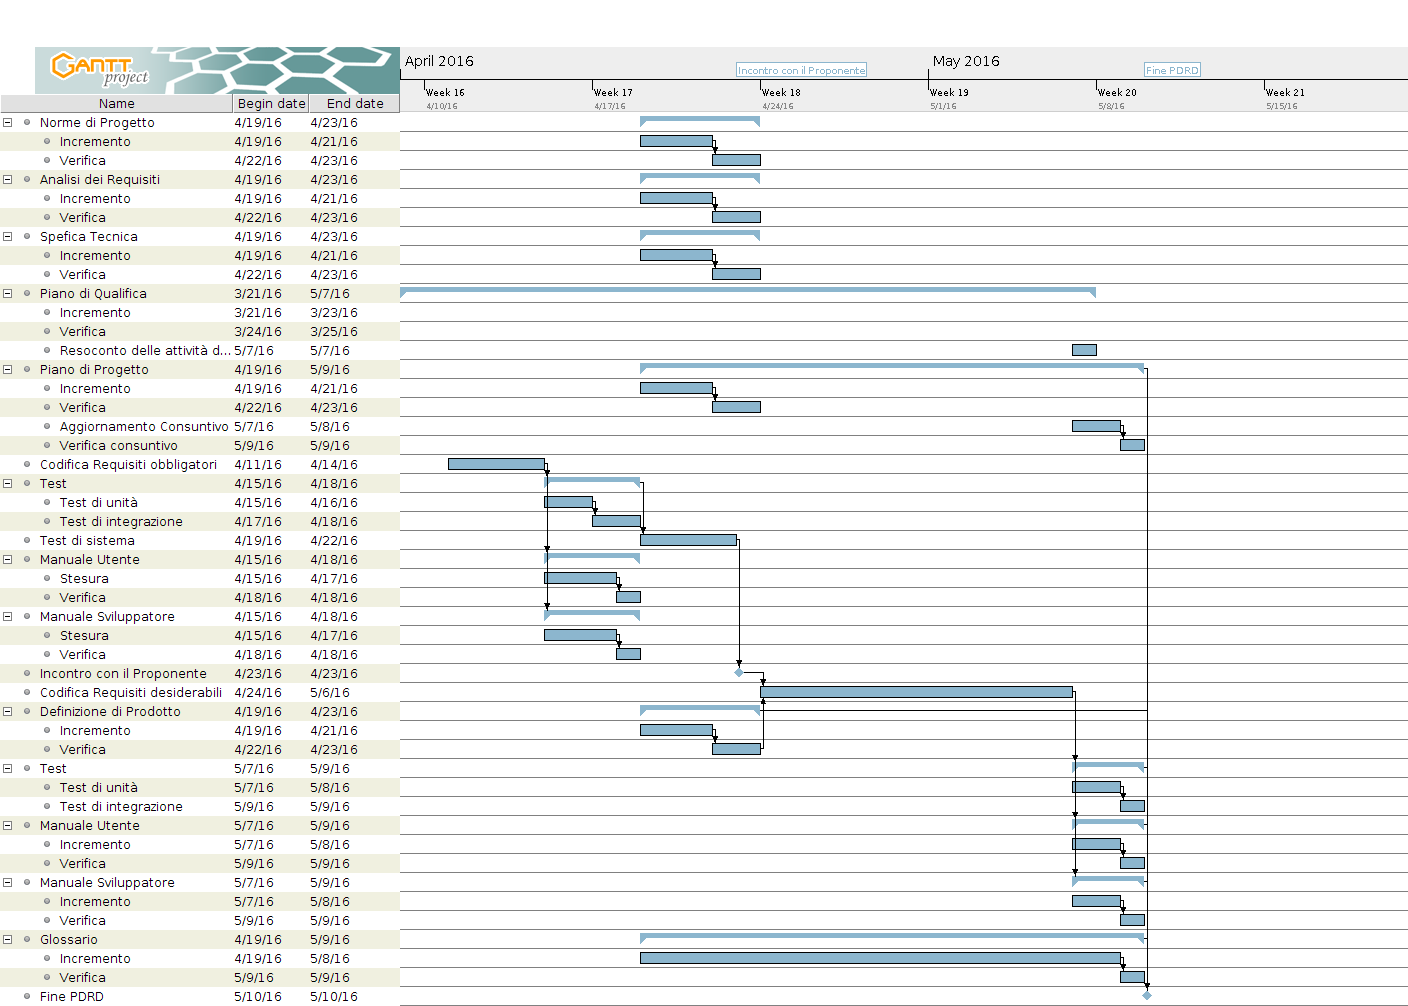
\includegraphics[width=\textwidth]{gantt_png/5-requisiti_desiderabili}
				\caption{Gantt - Fase PDRD}
				\label{fig:Gantt - Fase PDRD}
			\end{figure}
			

	\subsection{Fase PDROP: Progettazione di Dettaglio e codifica dei Requisiti Opzionali}
		\textbf{Periodo: dal 2016-05-15 al 2016-05-23}
		
		Questa fase\g\ comincia dopo la \revisionediqualifica\ e termina con la visione da parte del proponente del prototipo realizzato.

		Le attività di questa fase\g\ saranno le seguenti:
		\begin{itemize}
			
			\item codifica: con quest'attività inizia e termina lo sviluppo da parte dei programmatori dei requisiti opzionali. Sarà dunque seguito quanto riportato nel documento \textit{Definizione di prodotto v3.00};

			\item esecuzione test: verranno eseguiti automaticamente tutti i test di unità e di integrazione previsti dal documento \textit{Piano di Qualifica v6.00};

			\item manuale utente e manuale sviluppatore: continua la stesura dei manuali che forniranno indicazioni agli utilizzatori del sistema, aggiungendo le parti corrispondenti all'implementazione dei requisiti opzionali.

		\end{itemize}
		
		
		\subsubsection{Diagramma di Gantt – Fase PDROP}
			\begin{figure}[!h]
				\centering
				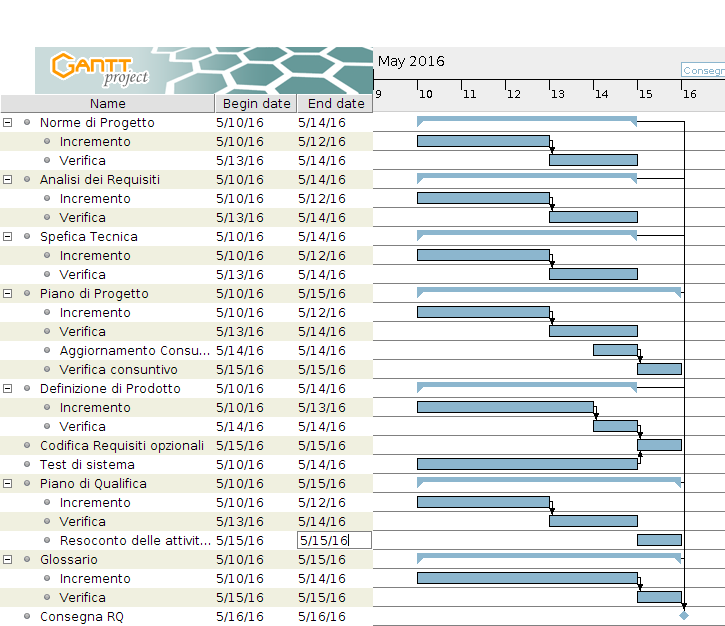
\includegraphics[width=\textwidth]{gantt_png/6-requisiti_facoltativi}
				\caption{Gantt - Fase PDROP}
				\label{fig:Gantt - Fase PDROP}
			\end{figure}
			
\newpage
	\subsection{Fase V: Validazione}
		\textbf{Periodo: dal 2016-05-24 al 2016-06-10}
		
		Questa fase\g\ comincia con la consegna della \revisionediqualifica\ e termina con la scadenza della consegna per la \revisionediaccettazione . Le principali attività di questa fase\g\ sono:

		\begin{itemize}
		
				\item incremento e verifica: se necessario verranno effettuati aggiornamenti ai vari documenti scritti;

				\item validazione: viene verificato, attraverso tracciamento, di aver soddisfatto i requisiti presenti nel documento \textit{Analisi dei requisiti v1.00};

				\item esecuzione test: verranno eseguiti i test di sistema previsti dal documento \textit{Piano di Qualifica v7.00};

				\item correzione bug\g : i bug\g\ rilevati verranno risolti;

				\item collaudo: viene eseguito un completo collaudo del sistema creato.
		\end{itemize}
		
		\subsubsection{Diagramma di Gantt – Fase V}
			\begin{figure}[!h]
				\centering
				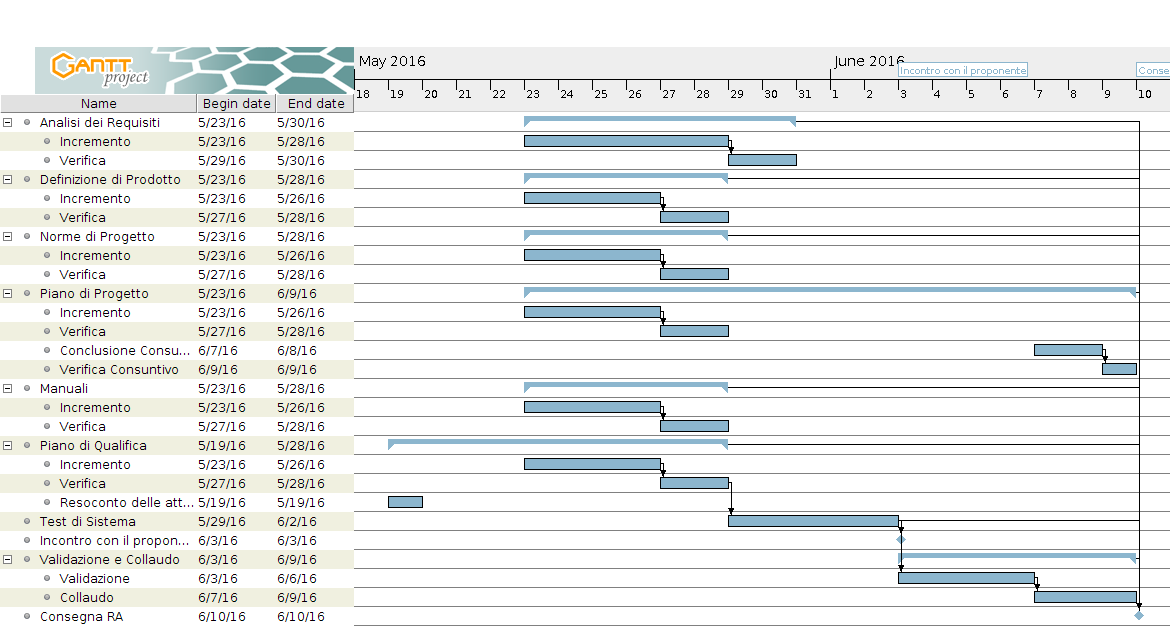
\includegraphics[width=\textwidth]{gantt_png/7-verifica}
				\caption{Gantt - Fase V}
				\label{fig:Gantt - Fase V}
			\end{figure}
			

\end{document}